\documentclass[xcolor=dvipsnames]{beamer} % Before typesetting your file, make sure PCTeX or whatever LaTeX software you are using is set to output a .pdf rather than the usual .dvi file.  
  \mode<presentation>
  \usetheme{Rochester}
\definecolor{GARNET}{RGB}{139, 19, 35}
\usecolortheme[named=GARNET]{structure} % you can change GARNET to any other color listed at http://en.wikibooks.org/wiki/LaTeX/Colors. Or you can ``define'' a color like I did for GARNET.



% Files needed are:
%    beamerposter.sty
%

%        \centering
%     {\tiny tiny}\par
%      {\scriptsize scriptsize}\par
%      {\normalsize normalsize}\par
%      {\large large}\par
%      {\Large Large}\par
%      {\LARGE LARGE}\par
%       {\huge huge}\par
%          {\Huge Huge}\par
%      {\veryHuge veryHuge}\par
%      {\VeryHuge VeryHuge}\par
%      {\VERYHuge VERYHuge}\par
%%%%%%%%%%%%%%%%%%%%%%%%
% The following commands affect the layout of the title bar.
\setbeamertemplate{headline}{  
  \leavevmode
  \begin{beamercolorbox}[wd=\paperwidth]{block title}
    \vspace{1cm}
        \center
        \usebeamercolor{title in headline}{\color{fg}{\Huge{\inserttitle}}\\[30pt]}
        \usebeamercolor{author in headline}{\color{fg}\Large{\insertauthor}\\[30pt]}
        \usebeamercolor{institute in headline}{\color{fg}\large{\insertinstitute}}     
    \vspace{1cm}
    
  \end{beamercolorbox}

  \begin{beamercolorbox}[wd=\paperwidth,ht=1cm,left]{headline}
        \includegraphics[width=10cm]
        {bates_Econ_logo.png} % Adjust the size and name of your logo file
        \vskip2cm
    \end{beamercolorbox}

  \begin{beamercolorbox}[wd=\paperwidth,ht=1cm,right]{headline}
        \includegraphics[width=10cm]
        {bates_college_seal_transparent_background.png} % Adjust the size and name of your logo file
        \vskip2cm
    \end{beamercolorbox}

}

%%%%%%%%%%%%%%%%%%%%%%%%%%%

\usepackage{times}
\usepackage{amsmath,amssymb}
\usepackage[english]{babel}
\usepackage[latin1]{inputenc}
\usepackage{url}
\usepackage[orientation=landscape,size=a0,scale=1.34,debug]{beamerposter} 
\usepackage{tikz}
\usepackage{hyperref}
\usepackage{biblatex}
\addbibresource{poster.bib}

%%%%%%%%%%%%%%%%%%%%%%%%%%%%%%

  \title{Unemployment insurance take-up on social networks}
  \author{Yuhao (Eric) Zhao, Advisor: Kyle Coombs}
  \institute{Economics Department, Bates College}

 

%%%%%%%%%%%%%%%%%%%%%%%%%%%%%%%%%%%%%%%%%%%%%%%%%%%%%%%%%%%%%%%%%%%%%%%%%%%%%%%%%%%%%%%%%%%%%%%%%%%%%%%%%%%%

\begin{document}
\begin{frame}{} 

  %%%%%%%%%%%%%%%%%%%%%%%%%%%%%%%%%%%%%%%%%%%%%%%%%%%%%%%%%%%%%%%%%%%%%%%%%%%%%%%%%%%%%%%%%%%%%%%%%%%%%%%%%%%%

\begin{columns}[t]

  %%%%%%%%%%%%%%%%%%%%%%%%%%%%%%%%%%%%%%%%%%%%%%%%%%%%%%%%%%%%%%%%%%%%%%%%%%%%%%%%%%%%%%%%%%%%%%%%%%%%%%%%%%%%



  \begin{column}{.3\linewidth} 
  
  \begin{block}{\LARGE Research Question}
  \begin{itemize}
        \vspace{0.3in}
      \item {\textbf{Motivation}}:
        \vspace{0.3in}
      \begin{enumerate}
        
      
      \item social capitals often plays essential roles in shaping how people make uses of other forms of capitals/resources through linkages and structures of social networks. 
      
      \item In terms of employment situations, it's generally assumed to be true that higher level of social capitals can lead to more efficient use of information about labor market and reduce the costs on both sides of the market.
      
      \item In studies of local social networks across developing countries, researchers have found significant results of informal insurance that embedded in people's social networks where insurance institutions are not been developed or much less accessible.
      
      \item We are curious about how the social networks affect the regional results of Unemployment Insurance (UI) benefit claim.

      

      
      \end{enumerate}
      \vspace{0.3 in}
      
      \item {\textbf{Question}}:
      \vspace{0.3in}
      
       My general question here is- \textit{Does aggregation of regional social capital through networks make up for unclaimed unemployment insurance benefits?}
  \end{itemize}
 
\end{block}

\begin{block}{ \LARGE Relevant Literature}
\begin{itemize}
    \vspace{0.3 in}
    \item {\textbf{Theory-based}}: 
    \vspace{0.3 in}
    \begin{enumerate}
        \item Networks in the Understanding of Economic Behaviors\cite{jackson2014networks}
        \item Informal insurance on social networks \cite{bloch2008informal}
        
    \end{enumerate}
    



\vspace{0.3 in}
    \item {\textbf{Empirical-based}}:
\vspace{0.3 in}
    \begin{enumerate}
        \item Social capital, friendship networks, and youth unemployment\cite{hallsten2017social}
        
        \item Macro-level analysis of social capital and unemployment in Europe \cite{freitag2011social}
        
        \item UI Take-up and eligibility  \cite{auray2020eligibility}

        \item  Social capital atlas project  \cite{chetty2022social1}\cite{chetty2022social2}

    \end{enumerate}
    

\end{itemize}

\end{block}


\begin{figure}[h]
\begin{minipage}{0.5\textwidth}
    \centering
    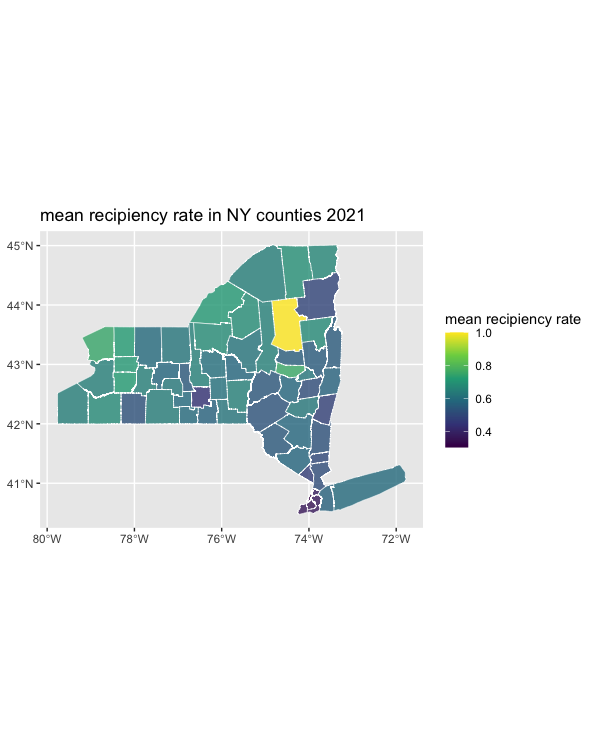
\includegraphics[width=\textwidth]{mean_recip_NY_2021.png} % First figure
  \end{minipage}\hfill
  \begin{minipage}{0.5\textwidth}
    \centering
    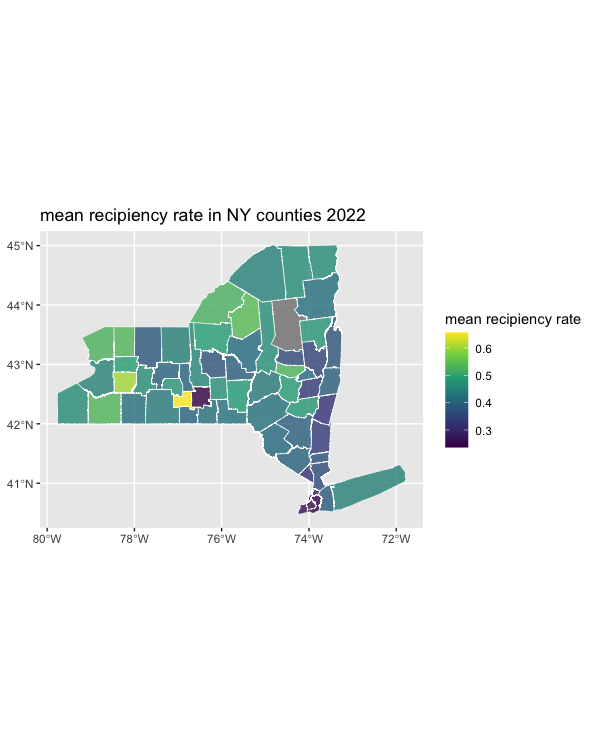
\includegraphics[width=\textwidth]{mean_recip_NY_2022.png} % Second figure
  \end{minipage}
\end{figure}

  \end{column}
  %%%%%%%%%%%%%%%%%%%%%%%%%%%%%%%%%%%%%%%%%%%%%%%%%%%%%%%%%%%%%%%%%%%%%%%%%%%%%%%%%%%%%%%%%%%%%%%%%%%%%%%%%%%%
  %%%%%%%%%%%%%%%%%%%%%%%%%%%%%%%%%%%%%%%%%%%%%%%%%%%%%%%%%%%%%%%%%%%%%%%%%%%%%%%%%%%%%%%%%%%%%%%%%%%%%%%%%%%%
  \begin{column}{.3\linewidth}



    \begin{block}{\LARGE Data}
\begin{itemize}
    \item Social Capital Data
    \begin{itemize}
        \item The social capital statistics come from the large-scale data project\href{https://socialcapital.org}{ Social Capital Atlas}. 
        \item The dataset is in cross-section data form where the first column is each US county and other columns are specific statistics using Facebook data (aged between 25 and 44 who reside in the United States, were active on the Facebook platform at least once in the prior 30 days, have at least 100 U.S.-based Facebook friends, and have a non-missing residential ZIP code as of May 2022) except population variables. 
        
    \end{itemize}

    \item  Unemployment and UI Data 

    \begin{itemize}
        \item The unemployment data we have collected is from New York Department of Labor's Local Area Unemployment Statistics program where it provides employment, unemployment, labor force, and unemployment rate data.

        \item We collect monthly data form across 63 counties in 2021-22. The variables include number of beneficiaries and total amount of benefits.

        

    \end{itemize}

\end{itemize}
 
    \end{block}



    \begin{block}{\LARGE Method}

    \begin{itemize}
        \item \textbf{Panel Data}:
        We select economic connectedness, fraction of closed triangles (clustering), volunteering rate from social capital data and UI data by year-month to construct the panel data.
        
        \item \textbf{Time Fixed-Effect}:
        Controlling for variables that are constant across entities but vary over time. 

       % Entity fixed effect:

       % Controlling for variables that vary across entities (Counties) constant over time.
       

        %Combined effect model:
        
       % The combined model allows to eliminate bias from unobservables that change over time but are constant over entities and it controls for factors that differ across entities but are constant over time. 
        
    \end{itemize}
    
    
      \end{block}

    \begin{block}{\LARGE Results}

 \begin{table}[h!]
   \centering
   \begin{tabular}{lccc}
      \tabularnewline \midrule \midrule
      Dependent Variable:  & \multicolumn{3}{c}{Average takeup rate}\\
      \hline
      Model:                       & (1)            & (2)            & (3)\\  
      \midrule
      \emph{Variables}\\
      Constant                     & 0.079          &                &   \\   
                                   & (0.060)        &                &   \\   
      ec\_county                   & -0.009         & -0.014         & -0.024\\   
                                   & (0.062)        & (0.053)        & (0.037)\\   
      clustering\_county           & 4.34$^{***}$   & 4.28$^{***}$   & 4.19$^{***}$\\   
                                   & (0.350)        & (0.318)        & (0.257)\\   
      volunteering\_rate\_county   & -0.496$^{**}$ & -0.484$^{**}$ & -0.464$^{***}$\\   
                                   & (0.188)        & (0.162)        & (0.102)\\   
      \midrule
      \emph{Fixed-effects}\\
      Year                         &                & Yes            & Yes\\  
      Month                        &                &                & Yes\\  
      \midrule
      \emph{Fit statistics}\\
      Observations                 & 1,454          & 1,454          & 1,454\\  
      R$^2$                        & 0.10077        & 0.31229        & 0.68439\\  
      Within R$^2$                 &                & 0.12503        & 0.23015\\  
      \midrule \midrule
      \multicolumn{4}{l}{\emph{Heteroskedasticity-robust standard-errors in parentheses}}\\
      \multicolumn{4}{l}{\emph{Signif. Codes: ***: 0.01, **: 0.05, *: 0.1}}\\
   \end{tabular}
\end{table}
        
    \end{block}


  \end{column}
  %%%%%%%%%%%%%%%%%%%%%%%%%%%%%%%%%%%%%%%%%%%%%%%%%%%%%%%%%%%%%%%%%%%%%%%%%%%%%%%%%%%%%%%%%%%%%%%%%%%%%%%%%%%%
  %%%%%%%%%%%%%%%%%%%%%%%%%%%%%%%%%%%%%%%%%%%%%%%%%%%%%%%%%%%%%%%%%%%%%%%%%%%%%%%%%%%%%%%%%%%%%%%%%%%%%%%%%%%%
  \begin{column}{.3\linewidth}
   


     %%%%%%%%%%%%%%%%%%%%%%%%%%%%%%%%%%%%%%%%%%%%%%%%%%%%%%%%%%%%%%%%%%%%%%%%%%%%%%%%%%%%%%%%%%%%%%%%%%%%%%%%%%%%
    \begin{block}{\LARGE Model}

Base Model:
$$Y_{\overline{takeup-rate}}=\alpha_i+\beta_1 X_{sec_{it}}+\beta_2 X_{clustering_{it}}+\beta_3 X_{vonluteering_{it}}+u_{it}$$

where $\alpha_i$ is the sum of constant term and unobserved entity-invariant heterogenities across time : $\alpha_i=\beta_0+\beta Z_i$
\vspace{0.2in}

The base model can be expressed as a regression model containing $n-1$ dummy regressors and a constant:

$$Y_{it}=\beta_0+\beta_1 X_{sec_{it}}+\beta_2 X_{clustering_{it}}+\beta_3 X_{vonlunteering_{it}} \\+\gamma_2 D2_t+\gamma_3 D3_t +...+\gamma_T DT_t+\mu_{it}$$
    \end{block}

\begin{block}{\LARGE Discussion}
\begin{itemize}
    \item The average level of individual EC (economic connectedness) of low-SES (below-median) members of that community doesn't really play roles in affecting the average UI take-up rates.
    
    \item Limitation on data availability and potential endogenity problems on social networks.  
\end{itemize}

\end{block}

\begin{block}{\LARGE Reference}
\printbibliography
    
\end{block}

\begin{block} {\LARGE Acknowledgement}
This work is inspired by Prof. Coombs' research on unemployment insurance and connections with my own research interests on social networks.

    
\end{block}

%\includegraphics[scale=1.2]{xy1}

%\includegraphics[scale=1.5]{ProdRule}

  \end{column}
  
  %%%%%%%%%%%%%%%%%%%%%%%%%%%%%%%%%%%%%%%%%%%%%%%%%%%%%%%%%%%%%%%%%%%%%%%%%%%%%%%%%%%%%%%%%%%%%%%%%%%%%%%%%%%%
  %%%%%%%%%%%%%%%%%%%%%%%%%%%%%%%%%%%%%%%%%%%%%%%%%%%%%%%%%%%%%%%%%%%%%%%%%%%%%%%%%%%%%%%%%%%%%%%%%%%%%%%%%%%%


\end{columns}

\end{frame}
\end{document}


